\textbf{{1.信号量及同步原语}}\\

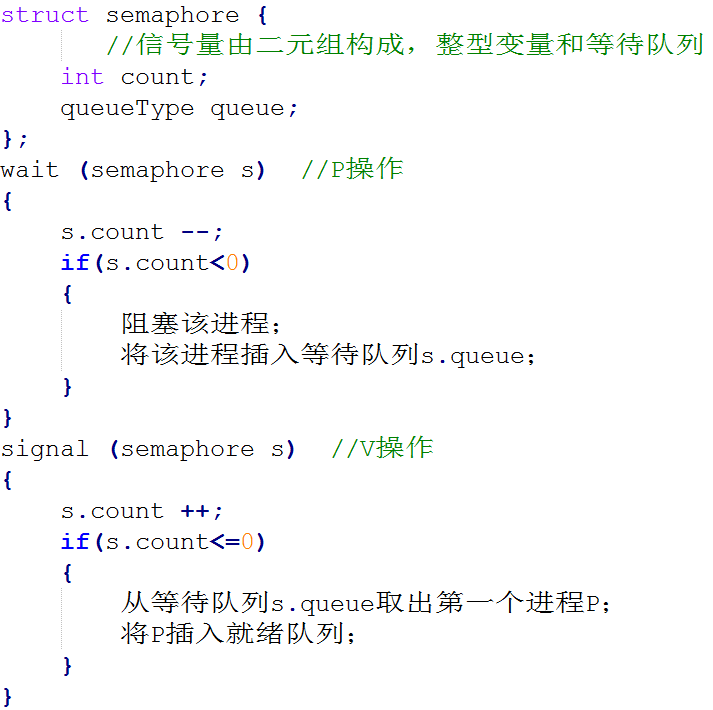
\includegraphics[width=6in]{png-jpeg-pics/31A68F58564D5473718C17263BC2F1D7.png}

\textbf{{P、V操作均为不可分割的原子操作}},这保证了对信号量进行操作过程中不会被打断或阻塞。P操作相当于申请资源,V操作相当于释放资源。P操作和V操作在系统中一定是成对出现,但未必在一个进程中,可以分布在不同进程中。

\textbf{{2.信号量的分类}}

\textbf{a.
整型信号量:}{整型信号量是一个整型量s,除初始化外,仅能通过标准的原子操作P和V来访问。整型信号量引入了P、V操作,但是在进行P操作时,如果无可用资源,则进程持续对该信号量进行测试,存在``忙等''现象,未遵循``让权等待''准则。}

\textbf{b. 记录型信号量(资源信号量)}

为了解决整型信号量存在的``忙等''问题,{\textbf{添加了链表结构}},用于链接所有等待该资源的进程,记录型信号量正是由于采用了记录型的数据结构而得名。\\

当进程对信号量进行P操作时,\textbf{若此时无剩余资源可用,则进程自我阻塞,放弃处理器,并插入到等待链表中}。可见,该机制遵循``让权等待''准则。当进程对信号量进行V操作时,若链表中仍有等待该资源的进程,则唤醒链表中的第一个等待进程。

\textbf{{3.信号量的应用}}{~}\textbf{{\\
}a.
实现进程同步:}假设存在并发进程P1和P2。P1中有一条语句S1,P2中有一条语句S2,要求S1必须在S2之前执行。这种同步问题使用信号量就很好解决。\\
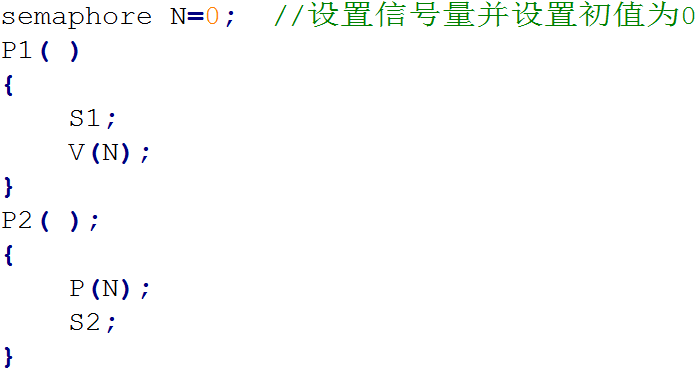
\includegraphics[width=3.33333in,height=1.79167in]{png-jpeg-pics/385B9D2BDF1FE32401CBDE9F621AB128.png}\\
\textbf{b.
实现进程互斥:}假设有进程P1和P2,两者有各自的临界区,但系统要求同时只能有一个进程进入自己的临界区,这里使用信号量可以很方便地解决临界区的互斥进入。设置信号量N,初值为1(即可用资源数为1),只需要将临界区放在P(N)和V(N)之间即可实现两进程的互斥进入。\\
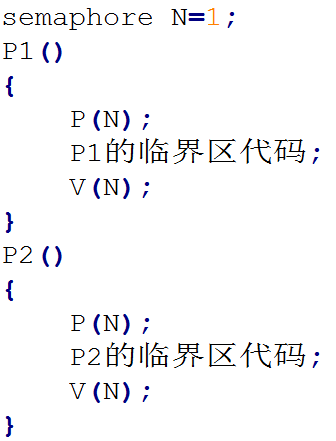
\includegraphics[width=1.87500in,height=2.45833in]{png-jpeg-pics/2DAFB1FCA7C1D490F4A0BD65E410DE83.png}\\

当有两个或者多个进程需要互斥访问某资源时,可以设置一个初值为1的信号量,在这些进程的访问资源的代码前后分别对该信号量进行P操作和V操作,即可保证进程对该资源的互斥访问。
